% !TEX TS-program = xelatex
% !TEX encoding = UTF-8
%
%
\documentclass[a4paper,12pt]{article}
\usepackage{ctex}
\usepackage{geometry,anysize,changepage,calc,hyperref,cite,fancyhdr,setspace}
\usepackage{amsmath,amssymb,amsthm,listings,xcolor}
\usepackage{graphicx,wrapfig,multirow,diagbox,caption, subcaption,verbatim}
\usepackage{caption,algorithm,algpseudocode}
\usepackage{url,natbib}
\usepackage{bm}
\bibliographystyle{abbrvnat}
\setcitestyle{open={(},authoryear,close={)}}
\renewcommand{\algorithmicrequire}{\textbf{输入}}
\renewcommand{\algorithmicensure}{\textbf{输出}}
\floatname{algorithm}{子程序}
\listfiles
%initialset.tex
%
\hypersetup{bookmarksopen=true,colorlinks=true,linkcolor=red,anchorcolor=blue,citecolor=green,linktocpage=true}
\captionsetup{font=footnotesize}
\captionsetup[sub]{font+=footnotesize}
\linespread{1.5}
\marginsize{2.13cm}{2.14cm}{2.4cm}{2.4cm}
\pagestyle{fancy}
\lstset{xleftmargin=1.5em,xrightmargin=1.5em,frame=lines}%,numbers=left,numberstyle=\tiny}
\chead{}\rhead{\thepage}\lhead{\leftmark}\cfoot{}\rfoot{}\lfoot{}

\newcommand{\vp}{\varphi}
\newcommand{\al}{\alpha}
\newcommand{\be}{\beta}
\newcommand{\ti}{\tilde}
\newcommand{\ve}{\varepsilon}
\newcommand{\de}{\delta}
\newcommand{\na}{\nabla}
\newcommand{\pd}{\partial}
\newcommand{\ud}{\mathrm{d}}
\newcommand{\mr}{\mathrm{R}}
\newcommand{\ms}{\mathbb{S}}
\newcommand{\mz}{\mathbb{Z}}
\newcommand{\mn}{\mathbb{N}}
\newcommand{\mc}{\mathbb{C}}
\newcommand{\one}{\textbf{1}}
\newcommand{\prox}{\textbf{prox}}
\DeclareMathOperator*{\argmax}{argmax}
\DeclareMathOperator*{\argmin}{argmin}
%\DeclareMathOperator*{\logg}{log}
%\DeclareMathOperator*{\det}{det}
\DeclareMathOperator*{\tr}{tr}
\DeclareMathOperator*{\st}{s.t.}

\theoremstyle{nonumberplain}
%\theoremheaderfont{\itshape}
%\theorembodyfont{\upshape}
%\theoremseparator{.}
%\theoremsymbol{\ensuremath{\square}
\newtheorem{definition}{定义}
\newtheorem{theorem}{定理}
\newtheorem{lemma}{引理}
%\newtheorem{proof}{证明}

%\renewcommand{\figurename}{{\zihao{5}图}}
%\renewcommand{\tablename}{{\zihao{5}表}}
%\makeatletter %下面两个命令用于创建非浮动体图表的标题
%  \newcommand\figcaption{\def\@captype{figure}\caption} 
%  \newcommand\tabcaption{\def\@captype{table}\caption} 
%\makeatother
%%\renewcommand{\abstractname}{摘\ 要}
%\renewcommand{\contentsname}{目\ 录}
%\renewcommand{\refname}{参考文献}

%\renewcommand{\thetable}{\arabic{section}.\arabic{table}}
%\renewcommand{\thefigure}{\arabic{section}.\arabic{figure}}
%\renewcommand{\theequation}{\arabic{section}.\arabic{equation}}

\makeatletter\@addtoreset{table}{section}\@addtoreset{figure}{section}\@addtoreset{equation}{section}\makeatother




\linespread{1.5}
\author{龙子超}
\title{{\heiti {\zihao{3} 数学分析II-习题课}}}
\date{}
\begin{document}
\maketitle
%===================正文====================
%\begin{abstract}
%\begin{spacing}{1.0}
%
%\end{spacing}
%\end{abstract}

%\tableofcontents
%\newpage

本习题答案集所给出的解答尽可能从教材出发. 课程教材为《数学分析》I-III, 伍胜健编著,
北京大学出版社.
\section*{2018-Mar-21}
\subsection*{作业}
\noindent III Chap13 18. 设函数$f(x,y)$在$\mathrm{R}^2$内除直线$x=a$与$y=b$外处处有定义,并且满足:
   \begin{enumerate}
     \itemsep-0.5em 
     \item $\lim_{y\to b}f(x,y)=g(x)$存在
     \item $\lim_{x\to a}f(x,y)=h(y)$一致存在, 即对于$\forall \varepsilon>0,\exists\delta>0,$
       使得对于$\forall (x,y)\in\{(x,y):0<|x-a|<\delta\}$有$|f(x,y)-h(y)|<\varepsilon$
   \end{enumerate}
   证明:存在$c\in\mathrm{R}$使得
   \begin{enumerate}
     \itemsep-0.5em 
     \item $\lim_{x\to a}\lim_{y\to b}f(x,y)=\lim_{x\to a}g(x)=c$
     \item $\lim_{y\to b}\lim_{x\to a}f(x,y)=\lim_{y\to b}h(y)=c$
     \item $\lim_{E\owns(x,y)\to(a,b)}f(x,y)=c$,其中$E=\mathrm{R}^2\setminus\{(x,y):x=a,or y=b\}$
   \end{enumerate}
\begin{proof}[提示]
  我们这里对一致存在做简单的解释: 这实际上是一致逼近的意思, 有兴趣的同学可以参考数分II第10章函数项级数的一致收敛的概念.

  将二元函数$f(x,y)$视作一系列一元函数$g_x(y)$, 对每个给定的$x\in\mr$, 
  我们定义一个一元函数, 记作$g_x:\mr\to\mr$, 
  \[g_x(y)=f(x,y),\forall y\in\mr\]

  于是随着$x$逼近$a$, 这一系列函数$g_x(h)$逼近$h(y)$. $\lim_{x\to a}f(x,y)=h(y)$
  一致存在的意思就是, 这一系列$g_x$是一致逼近$h$的: 也就是, 任给一个$\varepsilon$, 
  都存在一个$\delta_\varepsilon$, 只要$|x-a|<\delta_\varepsilon$, 都有$|g_x(y)-h(y)|<\varepsilon$

  举个例子:
  \begin{itemize}
    \itemsep-0.5em 
    \item $a=0,g_x(y)=x\ln y,x\in[0,1],y\in(0,1]$, 当$x\to0$时, 函数$g_x$逼近$h(y)\equiv0$, 但不是一致逼近的.如图\ref{fig:1}
    \item $a=0,g_x(y)=x+y,x\in[0,1],y\in[0,1]$, 当$x\to 0$时, 函数$g_x$逼近$h(y)=y$, 而且是一致逼近的.如图\ref{fig:2}
  \end{itemize}
  \begin{figure}[htbp]
    \centering 
    \begin{subfigure}{0.45\textwidth}
      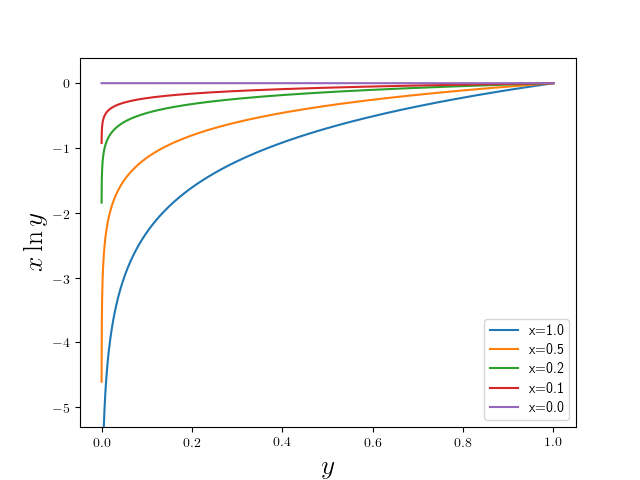
\includegraphics[width = \textwidth]{1.png}
      \caption{$g_x(y)=x\ln y$}
      \label{fig:1}
    \end{subfigure}
    \begin{subfigure}{0.45\textwidth}
      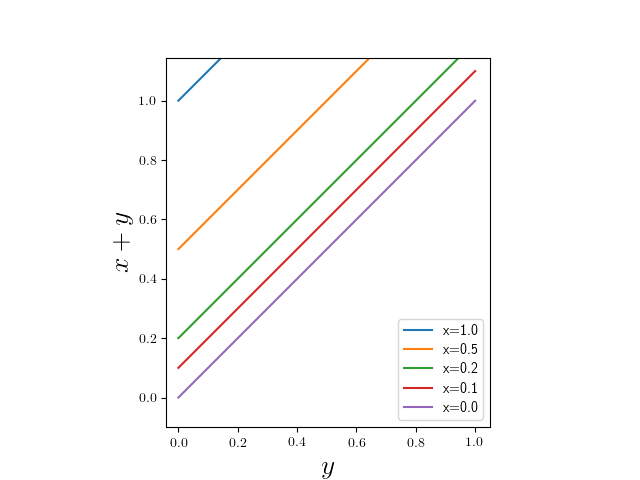
\includegraphics[width = \textwidth]{2.png}
      \caption{$g_x(y)=x+y$}
      \label{fig:2}
    \end{subfigure}
    \caption{}
  \end{figure}
\end{proof}


\noindent III Chap13 21. 设$E\subset\mathrm{R}^n$, 证明: 向量函数$\bm{f}(\bm{x}):E\to\mathrm{R}^m$
在$\bm{x}_0\in E$处连续的充分必要条件是对任何在$U(\bm{f}(\bm{x}_0),\delta)(\delta>0)$
内连续的函数$h(\bm{y}),h(\bm{f}(\bm{x}))$在$\bm{x}_0$处连续.
\begin{proof}\ 
  \begin{itemize}
    \item 必要性: 假设$h$在$U(\bm{f}(\bm{x}_0),\delta)$内连续,则容易验证
      $h(\bm{f})$在$\bm{x}_0$处连续
    \item 充分性: 假设对任何在$U(\bm{f}(\bm{x}_0),\delta)$内连续的函数$h$, $h(\bm{f})$在$\bm{x}_0$处都是连续的,
      那么$\bm{f}$一定在$\bm{x}_0$处连续. 否则, 存在一个大于0的常数$\varepsilon$及一系列趋近于$\bm{x}_0$的点$\{\bm{x}_n\}$, 
      使得$||\bm{f}(\bm{x}_n)-\bm{f}(\bm{x}_0)||>\varepsilon$, 取$h(\bm{u})=||\bm{u}-\bm{f}(\bm{x}_0)||^2$, 
      则$h(\bm{f}(\bm{x}_0))=0\in\mr^m,h(\bm{f}(\bm{x}_n))>\varepsilon^2$, 这与$h(\bm{f}(\bm{x}))$在$\bm{x}_0$处连续矛盾.
  \end{itemize}
\end{proof}

\noindent III Chap14 15. 设函数$u=f(\bm{x})$在$\bm{x}_0\in\mathrm{R}^n(n\geq2)$的邻域
$U(\bm{x}_0,\delta_0)$内存在$n$个偏导数, 且有$n-1$个偏导数在该邻域内连续. 
证明: $u=f(\bm{x})$在$\bm{x}_0$处可微.
\begin{proof}
  不妨设$\frac{\partial u}{\partial x_i},i=2,3,\cdots,n$在邻域内是连续的. 
  并假设$\bm{x}_0=(x_1^0,\cdots,x_n^0)$
  我们要证明
  \[f(\bm{x}_0+\Delta \bm{x})=f(\bm{x}_0)+\sum_{i=1}^{n}\frac{\partial f}{\partial x_i}\Delta x_i+o(|\Delta \bm{x}|)\]
  我们记$\bm{x}_0'=(x_2^0,\cdots,x_n^0), \Delta \bm{x}'=(\Delta x_2,\cdots,\Delta x_n)$, $g_{x_1}(\bm{x}')=f(x_1,\bm{x}')$.

  于是根据书中的定理14.1.2, 对邻域内的每个$x_1,g_{x_1}$在邻域内都是可微的.
  \begin{eqnarray*}
    f(\bm{x}_0+\Delta \bm{x})&=&f(x_1^0+\Delta x_1,\bm{x}_0')+\bm{D}g_{x_1^0+\Delta x_1}(\bm{x}_0')\Delta\bm{x}'+o(|\Delta\bm{x}'|)\\
    &=&f(x_1^0+\Delta x_1,\bm{x}_0')+\bm{D}g_{x_1^0}(\bm{x}_0')\Delta\bm{x}'+o(\bm{1})\cdot\Delta\bm{x}'+o(|\Delta\bm{x}'|)\\
    &=&f(\bm{x}_0)+\frac{\partial f}{\partial x_1}\Delta x_1+\bm{D}g_{x_1^0}(\bm{x}_0')\Delta\bm{x}'+o(\Delta x_1)+o(|\Delta\bm{x}'|)\\
    &=&f(\bm{x}_0)+\bm{D}f(\bm{x}_0)+o(|\Delta\bm{x}|)
  \end{eqnarray*}

  从而$f$在$\bm{x}_0$处是可微的.
\end{proof}
\noindent III Chap14 8. 设函数$z=u(x,y)$在$\mathrm{R}^2\setminus\{(0,0)\}$内可微, 令$x=r\cos\theta,y=r\sin\theta$, 在$Oxy$平面上作单位向量$e_{\bm{r}},e_{\bm{\theta}}$, 其中$e_{\bm{r}}$表示$\theta$固定时沿$r$增加的方向, $e_{\bm{\theta}}$表示$r$固定时沿$\theta$增加的方向. 证明:
\[\frac{\partial u}{\partial e_{\bm{r}}}=\frac{\partial u}{\partial r},\frac{\partial u}{\partial e_{\bm{\theta}}}=\frac{1}{r}\frac{\partial u}{\partial \theta}\]
\begin{proof}
  $(x,y)=(r\cos\theta,r\sin\theta)$, 因此
  \[
    \left\{
    \begin{array}{l}
    \ud x=\cos\theta\ud r-r\sin\theta\ud\theta,\\
    \ud y=\sin\theta\ud r+r\sin\theta\ud\theta
    \end{array}
    \right.\Rightarrow
    \left\{
      \begin{array}{l}
        \ud\theta=-\frac{\sin\theta}{r}\ud x+\frac{\cos\theta}{r}\ud y\\
        \ud r=\cos\theta\ud x+\sin\theta\ud y
      \end{array}
      \right.
  \]
\[\Rightarrow\left\{
  \begin{array}{l}
    \frac{\partial u}{\partial x}=-\frac{\sin\theta}{r}\frac{\partial u}{\partial \theta}+\cos\theta\frac{\partial u}{\partial r}\\
    \frac{\partial u}{\partial y}=\frac{\cos\theta}{r}\frac{\partial u}{\partial \theta}+\sin\theta\frac{\partial u}{\partial r}
  \end{array}\right.
    \]
    由于$e_{\bm{r}}=\frac{1}{r}(x,y),e_{\bm{\theta}}=\frac{1}{r}(-y,x)$, 利用上式对这两个方向求方向导数得:
  \[\Rightarrow\left\{
    \begin{array}{l}
      \frac{\partial u}{\partial e_{\bm{r}}}=(\frac{\partial u}{\partial x},\frac{\partial u}{\partial y})\cdot e_{\bm{r}}=\frac{\partial u}{\partial r}\\
      \frac{\partial u}{\partial e_{\bm{\theta}}}=(\frac{\partial u}{\partial x},\frac{\partial u}{\partial y})\cdot e_{\bm{\theta}}=\frac{1}{r}\frac{\partial u}{\partial \theta}
    \end{array}
    \right.
    \]
\end{proof}
\begin{proof}[讨论]
  对函数$f:\mr^n\to\mr$,及方向$\bm{v}$(不一定是单位向量),沿$\bm{v}$方向取微分/微元
  \[\ud f=\frac{\partial f}{\partial\bm{v}}\cdot[\bm{v}\cdot(\ud x_1,\cdots,\ud x_n)^\top]\]
  对函数$u=u(x_1,\cdots,x_n)$, $\frac{\partial u}{\partial \bm{x}}$在每个点局部定义了一个方向, 且沿此方向取微分/微元
  \[\ud f=\frac{\partial f}{\partial u}\cdot[\frac{\partial u}{\partial \bm{x}}\cdot(\ud x_1,\cdots,\ud x_n)^\top]\]
  因此, 若在某一点$\bm{v},\frac{\partial u}{\partial\bm{x}}$是同向的, 设$\bm{v}=\alpha\frac{\partial u}{\partial\bm{x}}$,则在这一点
  \[\frac{\partial f}{\partial\bm{v}}=\frac{1}{\alpha}\frac{\partial f}{\partial u}\]
\end{proof}

\subsection*{补充}
\noindent 1. 请举出一个函数$u=f(\bm{x})(\bm{x}\in\mathrm{R}^n)$,使得它同时满足下述条件:
\begin{enumerate}
  \itemsep-0.5em 
  \item $f(\bm{x})$在$\bm{x}=0$处各个方向导数都存在.
  \item $f(\bm{x})$在$\bm{x}=0$处各个偏导数都存在
  \item $f(\bm{x})$在$\bm{x}=0$处连续但不可微.
\end{enumerate}
\begin{proof}
  取$fx,y)=\sqrt{|xy|}$
\end{proof}

\noindent 2. 请举出一个函数$u=f(\bm{x})(\bm{x}\in\mathrm{R}^n)$,使得它同时满足下述条件:
\begin{enumerate}
  \itemsep-0.5em 
  \item $f(\bm{x})$在$\bm{x}=0$处可微
  \item $f(\bm{x})$在$\bm{x}=0$邻域内各方向导数存在
  \item $f(\bm{x})$在$\bm{x}=0$处偏导不连续
\end{enumerate}
\begin{proof}
  即作业题Chap14 10. 取$f(x,y)=(x^2+y^2)\sin\frac{1}{x^2+y^2}$
\end{proof}

\noindent 3. 复合函数求导: $\bm{g}:\mr^l\to\mr^m,\bm{f}:\mr^m\to\mr^n$在合适的邻域内连续可微.
记$\bm{u}(\bm{x})=\bm{f}(\bm{g}(\bm{x}))$, 则
\begin{eqnarray*}
  \ud\bm{u}&=&\bm{D}\bm{f}\ud\bm{g}\\
    &=& \bm{D}\bm{f}\bm{D}\bm{g}\ud\bm{x}
\end{eqnarray*}
因此$\bm{D}\bm{u}(\bm{x})=\bm{D}\bm{f}(\bm{g})\bm{D}\bm{g}(\bm{x})$, 即$\frac{\partial\bm{u}}{\partial\bm{x}}=\frac{\partial\bm{f}}{\partial\bm{g}}\cdot\frac{\partial\bm{g}}{\partial\bm{x}}$
\begin{enumerate}
  \itemsep-0.5em 
  \item $\bm{u}=\bm{f}(\cdots\bm{f}(\bm{f}(\bm{x}))\cdots)$, 其中$f:\mr^n\to\mr^n$. \\
    求$\frac{\partial\bm{u}}{\partial\bm{x}}$
  \item $\bm{u}=\bm{x}+\bm{f}(\bm{x},\bm{\theta})$, 其中$\bm{\theta}\in\mr^N,f(\cdot,\bm{\theta}):\mr^n\to\mr^n$.\\
    求$\frac{\partial\bm{u}}{\partial\bm{x}},\frac{\partial\bm{u}}{\partial\bm{\theta}}$
  \item $\bm{u}=\bm{x}+\bm{f}(\bm{x},\bm{\theta})+\bm{f}(\bm{f}(\bm{x},\bm{\theta}),\bm{\theta})$,其中$\bm{\theta}\in\mr^N,f(\cdot,\bm{\theta}):\mr^n\to\mr^n$\\
    求$\frac{\partial\bm{u}}{\partial\bm{x}},\frac{\partial\bm{u}}{\partial\bm{\theta}}$
\end{enumerate}
\begin{proof}
  略
\end{proof}


%\begin{algorithm}
%  \caption*{ADMM求解$\min_{X\succeq0}|X|_1,\st |SX-I|\leq\sigma$}
%  %  \caption{ADMM求解$\min_{X\succeq0}|X|_1,\st |SX-I|\leq\sigma$}\label{alg:ADMM}
%  \begin{algorithmic}
%    \Require $S,\sigma,\rho$
%    \Ensure $X,|X|_1$
%    \State \textbf{Repeat while not convergence}
%    \begin{enumerate}
%      \item  根据式(\ref{eq:updateW3_2}
%      $\sim$\ref{eq:updateZ3_2}),依次求$W^+,X^+,Y^+,Z^+$;
%      \item  根据式(\ref{eq:updateU3_2}),依次求${U^1}^+,{U^2}^+,{U^3}^+$;
%    \end{enumerate}
%    \Return $X,|X|_1$
%  \end{algorithmic}
%\end{algorithm}

%\begin{lstlisting}[language=Matlab,keywordstyle=\color{blue},commentstyle=\color{red!80!green!80!blue!80}, rulesepcolor=\color{red!50!green!50!blue!50},tabsize=4]
%
%\end{lstlisting}

%\begin{figure}[htbp!]
%\centering
%\makebox[\textwidth][c] {
%\includegraphics[width=0.9\paperwidth]{}
%}
%\caption{}\label{}
%\end{figure}
%
%\begin{figure}[htbp!]
%   \centering
%   \begin{subfigure}{.48\textwidth}
%	\centering
%	\includegraphics[width = \textwidth]{}
%	\caption{} \label{}
%   \end{subfigure} 
%   \begin{subfigure}{.48\textwidth}
%	\centering
%	\includegraphics[width = \textwidth]{}
%	\caption{} \label{}
%   \end{subfigure}
%   \caption{} \label{}
%\end{figure}

%\begin{table}[htbp!]
%\centering
%\caption{} 
%\begin{subfigure}{0.49\textwidth}
%   \centering
%   \caption{}
%   \begin{tabular}{}
%
%   \end{tabular}
%\end{subfigure}
%\begin{subfigure}{.49\textwidth}
%   \centering
%   \caption{} 
%   \begin{tabular}{}
%
%   \end{tabular}    
%\end{subfigure}
%\end{table}

%\begin{centering}
%\section*{致谢}\addcontentsline{toc}{section}{致谢}
%\end{centering}

%\newpage
%\begin{thebibliography}{}
%\addcontentsline{toc}{section}{参考文献}
%\bibitem{cite_ADMM}Boyd S, Parikh N, Chu E, et al. Distributed Optimization and Statistical Learning via the Alternating Direction Method of Multipliers[J]. Foundations \& Trends® in Machine Learning, 2011, 3(1):1-122.
%\bibitem{cite_FISTA}Beck A, Teboulle M. A Fast Iterative Shrinkage-Thresholding Algorithm for Linear Inverse Problems[J]. Siam Journal on Imaging Sciences, 2009, 2(1):183-202.
%\bibitem{cite_convexoptimization}Boyd S, Vandenberghe L. Convex Optimization[M]. Cambridge University Press, 2004.
%%\bibitem{cite_quasicrystalsgreen}刘有延,傅秀军.\emph{准晶体}[M]. 上海科技教育出版社,1999.
%\end{thebibliography}

\bibliography{ref}
\end{document}



